\section{Versuchsaufbau/-durchführung}\label{abs: aufbau}
In diesem Abschnitt werden die verwendeten Brückenschaltungen aufgeführt. Als Quelle für
die Speisespannung wurde in allen Versuchteilen ein Wechselstromgenerator mit variabler Frequenz
verwendet. \\
Zur Bestimmung eines unbekannten ohmschen Widerstandes, wird die Wheatonsche Brücke
benutzt (Abbildung \ref{fig: wheaton}).
Der Zusammenhang \eqref{eq: widerstandsbedingungen} vereinfacht sich in diesem Fall zu:
\begin{equation}
  R_{\symup{X}} = R_2 \frac{R_3}{R_4}
\end{equation}
Das Verhältnis $R_3 / R_4$ ist durch ein Potentiometer realisiert. Um eine Fehlerrechnung durchführen
zu können, wird der Widerstand $R_2$ drei mal varriert und jeweils die entsprechenden Werte für $R_3$, die
zum Verschwinden der Brückenspannung führen, aufgenommen. Als Nullindikator wird ein Oszilloskop verwendet. \\
Nach dem selben Prinzip werden die Kapazität eines Kondensators und dessen Wirkwiderstand bestimmt. Der Aufbau
der Kapazitätsmessbrücke ist in Abbildung \ref{fig: kapazität} dargestellt.

\begin{figure}
\centering
\begin{subfigure}{0.49\textwidth}
  \centering
  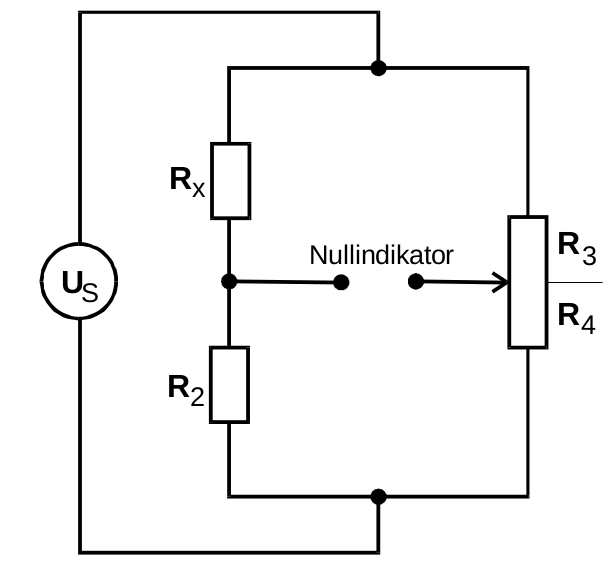
\includegraphics[width = 6cm]{pics/wheaton.png}
  \caption{Wheatonsche Brückenschaltung}
  \label{fig: wheaton}
\end{subfigure}
\begin{subfigure}{0.49\textwidth}
\centering
\includegraphics[width = 5.5cm]{pics/kap_brücke.png}
\caption{Kapazitätsmessbrücke}
\label{fig: kapazität}
\end{subfigure}
\caption{Wheaton- und Kapazitätsmessbrücke \cite{anleitung302}}
\label{fig: kapind}
\end{figure}

\begin{figure}
\centering
\begin{subfigure}{0.49\textwidth}
\centering
  \includegraphics[width = 4.6cm]{pics/ind_brücke.png}
\caption{Induktivitätsmessbrücke}
\label{fig: induktivität}
\end{subfigure}
\begin{subfigure}{0.49\textwidth}
  \centering
  \includegraphics[width = 6.8cm]{pics/max_brücke.png}
  \caption{Maxwell-Brücke}
  \label{fig: maxwell}
\end{subfigure}
\caption{Induktivitäts- und Maxwellmessbrücke\cite{anleitung302}}
\label{fig: indmax}
\end{figure}

Hierbei wird zunächst von einem idealen Kondensator ausgegangen, $R_x$ bzw. $R_2$ also aus der Schaltung entfernt. Für die
Kapazität $C_{\symup{X}}$ gilt in diesem Fall:
\begin{equation}
  C_{\symup{X}} = C_2 \frac{R_4}{R_3}
  \label{eq: Cx}
\end{equation}
Zur Bestimmung von $R_{\symup{X}}$ einer realen Kapazität wird als weiteres Stellglied der variable Widerstand $R_2$ in Reihe mit dem Kondesator $C_2$
geschaltet. Als weitere Bedingung für die Nullmethode neben \eqref{eq: Cx} ergibt sich:
\begin{equation}
  R_{\symup{X}} = R_2\frac{R_3}{R_4}
  \label{eq: Rx}
\end{equation}
Die Messung einer realen Induktivität wird zunächst mit einem Aufbau der Form \ref{fig: induktivität} durchgeführt.
Für $U_{\symup{Br}} = 0$ gelten hier die Bedingungen:
\begin{align}
  \begin{aligned}
    R_{\symup{X}} &= R_2\frac{R_3}{R_4} \\
    L_{\symup{X}} &= L_2\frac{R_3}{R_4}
  \end{aligned}
  \label{eq: Lx}
\end{align}

Anschließend geschieht die Induktivitätsmessung erneut mittels einer Maxwell-Brücke (siehe Abbildung \ref{fig: maxwell}).
Hierbei sind nun die Wiederstände $R_3$ und $R_4$ als unabhängige Stellglieder eingebaut. Die Bedingungen für die abgeglichene Brücke lauten
bei diesem Aufbau:
\begin{align}
  \begin{aligned}
    R_{\symup{X}} &=\frac{R_2 R_3}{R_4} \\
    L_{\symup{X}} &= R_2 R_3 C_4
  \end{aligned}
  \label{eq: Lx_maxwell}
\end{align}
Abschließend wird die Frequenzabhängigkeit einer Wien-Robinson-Brücke untersucht. Der Aufbau ist in Abbildung
 \ref{fig: wienrob} illustriert.
\begin{figure}
  \centering
  \includegraphics[width = 6cm]{pics/wien_rob_brücke.png}
  \caption{Wien-Robinson-Brücke\cite{anleitung302}}
  \label{fig: wienrob}
\end{figure}
Für das Verhältnis zwischen den Betragsquadraten der Speise- und Brückenspannung gilt:
\begin{equation}
  \left| \frac{\textfrak{U}_{\symup{Br}}}{\textfrak{U}_{\symup{S}}}\right|^2 = \frac{1}{9} \frac{(\Omega^2 - 1)^2 }{(1 - \Omega ^2)^2 + 9 \Omega ^2}
\end{equation}
Mit $\Omega = \frac{\omega}{\omega_0} = \omega R C$. Hierbei entspricht $\omega_0$ also der zu $\nu_0$ gehörigen Kreisfrequenz (siehe Abs. \ref{abs: theo}), die
für ein Verschwinden der Brückenspannung sorgt. Für variable Frequenzen $\nu \in [20, \num{30000}]\,\si{\hertz}$ werden $U_{\symup{S}}$ bzw. $U_{\symup{Br}}$ mit einem
Voltmeter bzw. der Peak-to-Peak-Einstellung des Oszilloskops gemessen. Die Untersuchung der Frequenzabhängigkeit
 ermöglicht in der Auswertung die Berechnung des Klirrfaktors \eqref{eq: klirr}.
